% =========================================================================
% How Robust Is the BLI Benefit? Global Sensitivity and Uncertainty
% Quantification of a Low-Order Power-Balance Model
%
% Draft for AIAA Journal of Propulsion and Power.
% NOTE: written against a generic article class for portability; port into
% the official AIAA "new-aiaa" template before submission (section text
% transfers unchanged).  Compile with:  latexmk -pdf main.tex
% or upload the paper/ directory to Overleaf.
%
% All quantitative claims are macros generated by studies/export_numbers.py
% (paper/numbers.tex) so the manuscript regenerates from the pipeline.
% =========================================================================
\documentclass[10pt]{article}

\usepackage[margin=1in]{geometry}
\usepackage{amsmath,amssymb}
\usepackage{graphicx}
\usepackage{booktabs}
\usepackage[round]{natbib}
\usepackage{xcolor}
\usepackage[colorlinks=true, allcolors=blue!50!black]{hyperref}
\usepackage{caption}
\captionsetup{font=small, labelfont=bf}

\graphicspath{{../figures/}}
% Auto-generated by studies/export_numbers.py -- do not edit.
\newcommand{\numReL}{2.28 \times 10^{8}}
\newcommand{\numVinf}{232.8}
\newcommand{\numthetaTE}{108}
\newcommand{\numHTE}{1.30}
\newcommand{\numdeltaFan}{0.65}
\newcommand{\numrHub}{0.56}
\newcommand{\numDragFus}{6.22}
\newcommand{\numPhiSurf}{1.32}
\newcommand{\numDEightPSC}{9.7\%}
\newcommand{\numDEightJet}{8.6\%}
\newcommand{\numDEightWake}{1.2\%}
\newcommand{\numDEightFPR}{1.034}
\newcommand{\numStarcFphi}{0.78}
\newcommand{\numStarcPSC}{13.9\%}
\newcommand{\numStarcPSCshaft}{12.3\%}
\newcommand{\numStarcNetMech}{4.0\%}
\newcommand{\numStarcNetElec}{1.53\%}
\newcommand{\numStarcFuel}{-1.88\%}
\newcommand{\numStarcFuelNoSnow}{-1.40\%}
\newcommand{\numStarcDtot}{27.5}
\newcommand{\numStarcDfus}{6.22}
\newcommand{\numSmithErr}{0.00\%}
\newcommand{\numUQPscMean}{18.4\%}
\newcommand{\numUQPscSd}{5.2\%}
\newcommand{\numUQPscPlo}{11.0\%}
\newcommand{\numUQPscPmed}{17.6\%}
\newcommand{\numUQPscPhi}{27.8\%}
\newcommand{\numUQNetPlo}{0.23\%}
\newcommand{\numUQNetPmed}{1.57\%}
\newcommand{\numUQNetPhi}{2.96\%}
\newcommand{\numUQFuelPlo}{-3.71\%}
\newcommand{\numUQFuelPmed}{-1.96\%}
\newcommand{\numUQFuelPhi}{-0.29\%}
\newcommand{\numSobolAeroTopName}{$f_\Phi$}
\newcommand{\numSobolAeroTopVal}{0.83}
\newcommand{\numSobolAeroSecondName}{$n$}
\newcommand{\numSobolAeroSecondVal}{0.14}
\newcommand{\numSobolNetTopName}{$\eta_{elec}$}
\newcommand{\numSobolNetTopVal}{0.49}
\newcommand{\numSobolNetSecondName}{$f_\Phi$}
\newcommand{\numSobolNetSecondVal}{0.45}
\newcommand{\numSobolFuelTopName}{$\eta_{elec}$}
\newcommand{\numSobolFuelTopVal}{0.49}
\newcommand{\numSobolFuelSecondName}{$f_\Phi$}
\newcommand{\numSobolFuelSecondVal}{0.45}
\newcommand{\numSobolCondElec}{0.53}
\newcommand{\numSobolCondFphi}{0.20}
\newcommand{\numSobolCondN}{0.22}
\newcommand{\numSobolCondKdist}{0.14}
\newcommand{\numSobolCondFpr}{0.06}


\title{How Robust Is the BLI Benefit?\\
\large Global Sensitivity and Uncertainty Quantification of a Low-Order
Power-Balance Model}
\author{Ansh Pathak\thanks{The Resonance Foundation,
administrator@theresonancefoundation.org;
draft prepared with AI assistance under human direction --- see the
acknowledgments and data-availability statements.}}
\date{Draft of \today}

\begin{document}
\maketitle

% -------------------------------------------------------------------------
\begin{abstract}
\noindent
Published estimates of the boundary-layer-ingestion (BLI) propulsion benefit
for transport aircraft span 2--12\,\% and are frequently contradictory,
because they measure different quantities under different bookkeeping rules
and almost never report uncertainty. This paper presents \texttt{blipb},
to our knowledge the first open-source, tested implementation of the Drela
power-balance BLI
benefit model, unifying the Smith (1993) wake-ingestion analysis and the
Hall et al.\ (2017) dissipation decomposition in one reproducible pipeline,
and subjects it to formal global sensitivity analysis and uncertainty
quantification. The model chains an axisymmetric integral boundary-layer
solver to a two-case podded-versus-BLI comparator whose energy bookkeeping
satisfies an exact ledger identity ($P_{K,\mathrm{pod}}-P_{K,\mathrm{BLI}}
=\Delta\Phi_{\mathrm{jet}}+\Delta\Phi_{\mathrm{wake}}$, enforced to
$10^{-10}$ in continuous integration), a compressible fan with an explicit
distortion penalty, a turboelectric chain, and Breguet mission accounting.
Validation reproduces the Smith analytic limit to \numSmithErr, the D8
wind-tunnel benefit to within 1.6 percentage points with a mechanistic
diagnosis of the difference, and brackets the published STARC-ABL
assessments. Across the seven-dimensional design/uncertainty space, the
5th--95th percentile band of the aerodynamic power-saving coefficient is
[\numUQPscPlo, \numUQPscPhi], and the net block-fuel benefit of a
STARC-ABL-class turboelectric installation is [\numUQFuelPlo,
\numUQFuelPhi]. The net benefit exhibits an interior optimum near
$f_\Phi\approx0.55$ --- full ingestion is a net penalty at realistic
distortion sensitivities --- and conditional Sobol' indices show that once
the captured dissipation fraction exceeds 0.5, electrical-chain efficiency
($S_T=0.53$) and fan-face profile shape (0.22) --- not further ingestion
(0.20) --- dominate the variance of the delivered benefit. Code, data and
every figure regenerate from an archived repository.
\end{abstract}

% -------------------------------------------------------------------------
\section{Introduction}\label{sec:intro}

Boundary-layer ingestion is among the few remaining airframe--propulsion
integration measures projected to reduce transport-aircraft fuel burn by
whole percentage points, and it occupies a central place in NASA's N+3
studies and their European counterparts \citep{welstead2016, seitz2021,
kim2014}. The physical idea is classical \citep{smith1993}: a propulsor that
ingests the low-momentum air of the airframe's boundary layer needs a
smaller jet velocity increment to produce the same net force, so it deposits
less kinetic energy into the atmosphere and requires less mechanical power.
The engineering question --- \emph{how large is the benefit for a realistic
configuration, and how confident are we in that number?} --- has proven
stubbornly difficult, for three reasons.

First, the benefit resists conventional bookkeeping. For a BLI
configuration the airframe wake and the propulsive jet occupy a shared
stream tube, so the split of the streamwise force into ``thrust'' and
``drag'' is a modeling convention, not a measurable \citep{drela2009}.
Different conventions yield different benefit numbers from identical flow
fields, and the literature contains examples of each. \citet{drela2009}
resolved the ambiguity by replacing the force ledger with a mechanical
energy ledger --- the \emph{power balance} --- in which only scalar,
positive-definite power and dissipation terms appear and no thrust/drag
split is ever performed. The power balance has since become the standard
language of BLI benefit analysis \citep{hall2017, uranga2017}.

Second, the published record is scattered. The STARC-ABL single-aisle
turboelectric concept was introduced with a 12\,\% design-mission fuel
benefit \citep{welstead2016}; the revised NASA assessment reports 3.4\,\%
\citep{felder2022}; coupled RANS/cycle optimization reports a 2.1--2.3\,\%
power saving \citep{yildirim2022}; and an independent industrial assessment
of the propulsive-fuselage class concludes the benefit can be a
\emph{penalty} of $+1.7\pm1.0$\,\% once electrical-chain and installation
masses are honestly counted \citep{giannakakis2020}. The one high-quality
experiment, the MIT/Aurora D8 campaign, measured $8.2\pm0.8$\,\% mechanical
flow-power saving at tunnel scale \citep{uranga2017}, decomposed by
\citet{hall2017} into jet (5.2\,\%), surface (2.4\,\%) and wake (0.6\,\%)
dissipation mechanisms. Recent reviews \citep{moirou2023, ma2025} emphasize
that these numbers measure \emph{different quantities under different
rules}, and call explicitly for reconciliation in a common framework.

Third --- and this is the gap this paper addresses --- the field has
essentially no uncertainty quantification. High-fidelity studies
\citep{yildirim2022, gray2018} are structurally unable to sweep the joint
design/uncertainty space (each point is a RANS solve), and the low-order
studies that could afford it have not done it. The D8 experiment's
$\pm0.8$\,\% is instrument-error propagation, not model uncertainty. No
peer-reviewed publication reports Sobol' importance rankings or output
probability distributions for the BLI benefit; no open-source implementation
of the power-balance benefit model exists against which such an analysis
could be reproduced. General conceptual-design frameworks (NASA Aviary,
OpenConcept, SUAVE/RCAIDE) treat BLI, when at all, as an assumed coupling
coefficient rather than a dissipation ledger.

This paper makes four contributions. \textbf{(i)}~It shows that the Smith
(1993), Drela (2009) and Hall (2017) formulations are consistent limits of
one implementation: the comparator's saving decomposes \emph{exactly} into
jet-mixing and wake-mixing dissipation terms (an algebraic identity proved
in Appendix~A and enforced to $10^{-10}$ relative in continuous
integration), and reproduces Smith's analytic wake-ingestion limits to
\numSmithErr. \textbf{(ii)}~It releases \texttt{blipb}, to our knowledge the
first open-source, pip-installable, tested implementation of the
power-balance BLI benefit model, with per-rule validations against the D8
measurement and the STARC-ABL assessments. \textbf{(iii)}~It reports, for
the first time, formal variance-based global sensitivity indices and
Monte-Carlo uncertainty bands for the BLI benefit over the joint
design/uncertainty space of a STARC-ABL-class installation.
\textbf{(iv)}~It provides a parametric benefit atlas from which a conceptual
designer can read the expected saving with confidence bands for a chosen
ingestion fraction, fan pressure ratio and mission, including an explicit
account of a bookkeeping subtlety --- the \emph{dilution effect} --- that
makes the per-propulsor benefit ratio \emph{fall} with ingestion fraction
even as the raw aircraft-level saving grows, while the \emph{net} saving
peaks at intermediate ingestion and collapses beyond it
(Section~\ref{sec:atlas}).

Section~\ref{sec:method} develops the model; Section~\ref{sec:vv} verifies
and validates it; Section~\ref{sec:atlas} presents the parametric atlas;
Section~\ref{sec:uq} the sensitivity and uncertainty results;
Section~\ref{sec:discussion} the limitations and the comparison with
high-fidelity results; Section~\ref{sec:conclusions} concludes.

% -------------------------------------------------------------------------
\section{Method}\label{sec:method}

\subsection{Power-balance framework}\label{sec:powerbalance}

Drela's power balance \citep{drela2009} integrates the mechanical-energy
equation over a control volume bounded by the vehicle surface, a downstream
Trefftz plane where static pressure has relaxed to $p_\infty$, and lateral
boundaries at freestream conditions. At unaccelerated level cruise the
balance reduces to: the mechanical flow power $P_K$ delivered through the
propulsor planes equals the sum of all dissipation inside the volume plus
the kinetic-energy flux deposited through the Trefftz plane, with no thrust
or drag appearing anywhere. Two properties make it the correct language for
BLI. First, every term is a scalar power with a definite sign, so
double-counting is structurally visible. Second, the kinetic-energy
thickness $\theta^*$ of a boundary layer obeys
%
\begin{equation}
  \tfrac12 \rho_e u_e^3\,\theta^*(x) \;=\; \Phi(x),
  \label{eq:kethickness}
\end{equation}
%
the cumulative viscous dissipation upstream of station $x$: the boundary
layer carries an integrated ledger of the energy already lost, which is
exactly the quantity an ingesting propulsor can partially recover. Our
implementation evaluates the ledger at a single canonical reference state
(the freestream-static condition), encoded as a frozen \texttt{ControlVolume}
object shared by construction between the two compared cases --- an
inconsistent comparison is a type error, not a silent bias.
Figure~\ref{fig:schematic} shows the control volume and the ledger terms.

\begin{figure}[t]
  \centering
  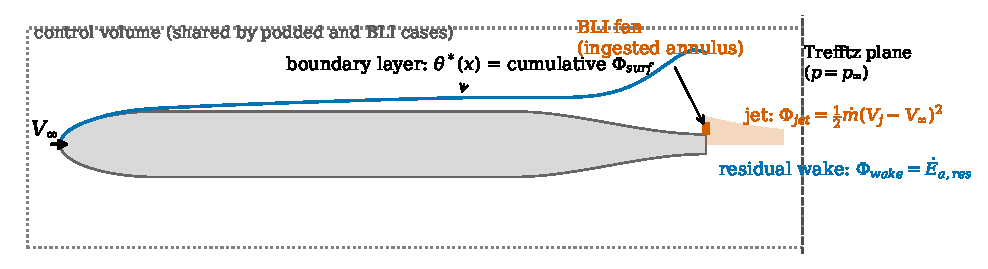
\includegraphics[width=0.95\linewidth]{fig1_schematic.pdf}
  \caption{Power-balance control volume shared by the podded and BLI cases:
  the fuselage boundary layer carries the cumulative surface dissipation
  $\theta^*(x)$ to the tail-cone fan face; the ledger splits the delivered
  mechanical flow power between jet-mixing dissipation and the residual
  wake at the Trefftz plane.}
  \label{fig:schematic}
\end{figure}

\subsection{The two-case comparator}\label{sec:comparator}

The benefit is computed by direct evaluation of two cases from one shared
parameter set, at equal net streamwise force, equal flight condition, equal
fan pressure ratio (FPR) and equal fan technology, differing only in what
the fan inhales.

\paragraph{BLI case.} The fuselage boundary layer arriving at the tail-cone
fan face is represented by a power-law profile $u/V_\infty=(y/\delta)^{1/n}$
on the annulus around the hub radius $r_{\mathrm{hub}}$, with $\delta$ sized
so the annulus carries exactly the momentum-defect flux delivered by the
boundary-layer solver (Section~\ref{sec:ibl}); the transverse-curvature
(thick-layer) effect on the tail cone is thereby consistent with the drag
bookkeeping by construction. A capture height $y_c$ ingests the Hall
dissipation fraction
%
\begin{equation}
  f_\Phi(y_c) \;=\;
  \frac{\int_0^{y_c} u\,(V_\infty^2-u^2)\,(r_{\mathrm{hub}}+y)\,dy}
       {\int_0^{\delta} u\,(V_\infty^2-u^2)\,(r_{\mathrm{hub}}+y)\,dy},
  \label{eq:fphi}
\end{equation}
%
the fraction of the layer's kinetic-energy defect --- equivalently, by
Eq.~\eqref{eq:kethickness}, of the cumulative upstream surface dissipation
footprint --- swallowed by the fan. An adiabatic boundary layer preserves
total temperature while destroying total pressure, so the fan inherits
$T_{t,\mathrm{in}}=T_{t\infty}$ but a mass-averaged
$\bar p_{t,\mathrm{in}}<p_{t\infty}$; applying the FPR to this degraded
inlet automatically produces the lower jet velocity $V_j'$ that constitutes
the BLI advantage. The fan model is one-dimensional and compressible with
polytropic efficiency $\eta_{\mathrm{pol}}$ reduced by an explicit
distortion penalty $\delta\eta = k_{\mathrm{dist}} f_\Phi$
\citep{fidalgo2012, gray2018}. The mechanical flow power is the
mechanical-energy flux added between the fan planes,
$P_{K,\mathrm{BLI}} = \tfrac12\dot m (V_j'^2 - V_\infty^2) -
\dot E_{\mathrm{exc}}$, where
$\dot E_{\mathrm{exc}}=\tfrac{\rho}{2}\!\int u\,(u^2-V_\infty^2)\,dA<0$ is
the ingested kinetic-energy-flux excess.

\paragraph{Podded reference.} The same fan at the same FPR inhales clean
freestream air ($p_{t\infty}$, $T_{t\infty}$) and its mass flow is sized in
closed form so the (fuselage + propulsor) subsystem produces the identical
net streamwise force, the full fuselage wake now left to dissipate:
$\dot m_{\mathrm{pod}} = (S + \dot D_{\mathrm{full}})/(V_j - V_\infty)$,
with $S$ the subsystem force of the BLI case and $\dot D_{\mathrm{full}}$
the total momentum-defect flux. The power-saving coefficient is
$\mathrm{PSC} = 1 - P_{K,\mathrm{BLI}} / P_{K,\mathrm{pod}}$.

\paragraph{Exact ledger identity.} Appendix~A shows, by rearrangement of
the defect integrals only --- valid for \emph{any} jet velocities the fan
model produces --- that
%
\begin{equation}
  P_{K,\mathrm{pod}} - P_{K,\mathrm{BLI}}
  \;=\;
  \underbrace{\left(\Phi_{\mathrm{jet}}^{\mathrm{pod}}
    - \Phi_{\mathrm{jet}}^{\mathrm{BLI}}\right)}_{\Delta\Phi_{\mathrm{jet}}}
  \;+\;
  \underbrace{\tfrac{\rho}{2}\!\int_{\mathrm{ingested}}\!
    u\,(V_\infty-u)^2\,dA}_{\Delta\Phi_{\mathrm{wake}} = \dot E_{a,\mathrm{ing}}},
  \label{eq:ledger}
\end{equation}
%
with $\Phi_{\mathrm{jet}}=\tfrac12\dot m (V_j-V_\infty)^2$ the eventual
jet-mixing dissipation. Equation~\eqref{eq:ledger} \emph{is} the
Drela--Hall decomposition: the entire saving is the reduced jet-mixing loss
plus the ingested wake-mixing loss that no longer occurs. Because the
identity is algebraically exact, it functions as an automated
bookkeeping-residual test: every comparator evaluation asserts it to
$10^{-10}$ relative (observed residuals are at machine precision,
$\mathcal{O}(10^{-16})$), and any future modification that breaks energy
accounting fails the continuous-integration suite loudly. This addresses
the double-counting and control-volume-inconsistency pitfalls that reviews
identify as the dominant error sources in low-order BLI studies
\citep{moirou2023}.

\subsection{Relation to the Smith and Hall formulations}\label{sec:unification}

Smith's wake-ingestion analysis \citep{smith1993} emerges as the ideal-fan,
incompressible, uniform-wake limit. For full ingestion of a uniform wake of
velocity ratio $w=V_w/V_\infty$ at the self-propelled condition, the ledger
gives the closed form $\mathrm{PSC} = 2(1-w)/(3-w)$, and for arbitrary
profiles a closed form in the profile's defect integrals
(Section~\ref{sec:vv}). The Hall decomposition is Eq.~\eqref{eq:ledger}
itself; the effective fill factor $\eta_{\mathrm{fill}}$ of the compact
estimator $\mathrm{PSC}\simeq f_\Phi\,\eta_{\mathrm{fill}}
(V_j-V_w)/(V_j+V_\infty)$ is recovered from the comparator as the achieved
fraction of the ideally recoverable power. All three formulations therefore
coexist as views of one computation rather than as competing models.

\subsection{Integral boundary-layer chain}\label{sec:ibl}

The fuselage is a body of revolution (elliptic nose, cylindrical midbody,
cubic tail-cone contraction to the fan hub radius); the inviscid
edge-velocity distribution comes from the classical von K\'arm\'an axial
source-line method with a G\"othert-type subsonic correction, blended into a
stagnation ramp over the inner nose where the slender-body approximation
fails. The boundary layer is marched with Thwaites' method
\citep{thwaites1949} in Mangler (axisymmetric) form \citep{mangler1948}
over the laminar run, switched at forced or Michel-criterion transition
\citep{michel1951} (whichever is earlier;
$x_{tr}/L$ is a UQ variable), and continued with Head's entrainment method
\citep{head1958, cebeci1977} carrying the thin-layer axisymmetric metric
terms, Ludwieg--Tillmann skin friction \citep{ludwieg1950}, and an
adiabatic-wall compressibility factor equivalent to Van~Driest~II within
$\sim$1\,\% for $M_e<1$ \citep{vandriest1956}. The kinetic-energy thickness
is reconstructed algebraically from the XFOIL-family shape-factor closure
$H^*(H, Re_\theta)$ \citep{drela1987}, giving the cumulative dissipation by
Eq.~\eqref{eq:kethickness} without a lag equation. The trailing-edge state
is carried to the freestream-static reference station by the Squire--Young
closure \citep{squireyoung1938} applied to the momentum-defect area
$r\theta$. Solutions with $H>2.4$ anywhere on the body are flagged invalid
and excluded from all maps --- never silently plotted.

At the frozen baseline (Table~\ref{tab:baseline}: $M_\infty=0.785$,
FL350, $L=37$\,m, $Re_L=\numReL$), the chain yields a trailing-edge momentum
thickness of \numthetaTE\,mm, shape factor \numHTE, fan-face profile
thickness $\delta=\numdeltaFan$\,m on a hub of $r_{\mathrm{hub}}
=\numrHub$\,m, fuselage drag \numDragFus\,kN and surface dissipation
\numPhiSurf\,MW --- a boundary layer of the same order as the fan radius,
which is precisely the STARC-ABL regime.

\begin{table}[t]
\centering\small
\caption{Frozen baseline (SPEC.md v1.0 with logged amendments).}
\label{tab:baseline}
\begin{tabular}{ll}
\toprule
cruise & $M_\infty=0.785$ at FL350 (ISA) \\
fuselage & $L=37$\,m, $D=3.76$\,m, tail radius $0.30\,r_{\max}$ \\
Reynolds number & $Re_L = \numReL$ \\
aft fan & FPR 1.25 baseline, $\eta_{\mathrm{pol}}=0.92$, $k_{\mathrm{dist}}=0.03$ \\
aircraft & $W=60$\,t, $L/D=21.4$, TSFC $14.2$\,mg/(N\,s) \\
turboelectric chain & $\eta_{\mathrm{elec}}=0.92$ baseline \\
mission & 500--3500\,nmi, snowball 1.35 \\
\bottomrule
\end{tabular}
\end{table}

\subsection{Propulsion chain and mission}\label{sec:mission}

The aircraft-level net saving charges the aft propulsor's shaft power with
the turboelectric transmission loss and normalizes by the total propulsive
shaft power of the aircraft,
%
\begin{equation}
  \mathrm{PSC}_{\mathrm{net}} =
  \frac{P_{\mathrm{sh,pod}} - P_{\mathrm{sh,BLI}}/\eta_{\mathrm{elec}}}
       {P_{\mathrm{sh,total}}},
  \qquad
  P_{\mathrm{sh,total}} = \frac{D_{\mathrm{total}} V_\infty}{\eta_{\mathrm{prop}}},
  \label{eq:netpsc}
\end{equation}
%
with $D_{\mathrm{total}} = W g/(L/D)$ and $\eta_{\mathrm{prop}}=0.80$ for
the underwing turbofans; setting $\eta_{\mathrm{elec}}=1$ recovers a
mechanically driven fan (D8-style architecture). The BLI power fraction is
thus \emph{dynamic} --- it grows with the captured stream tube --- rather
than frozen at a design-point value, keeping ingestion sweeps physically
consistent. Block fuel follows Breguet at fixed range with the effective
TSFC scaled by $(1-\mathrm{PSC}_{\mathrm{net}})$ and an empty-weight
snowball factor of 1.35 for rubber-airframe accounting.

\subsection{Implementation and reproducibility}

The pipeline is pure Python (\texttt{numpy}/\texttt{scipy} numerics,
\texttt{SALib} \citep{herman2017} and \texttt{chaospy} \citep{feinberg2015}
for UQ) with 63 unit/verification tests at 90\,\% line coverage, continuous
integration on Linux/macOS/Windows, and pinned environments
(\texttt{uv.lock}). A single boundary-layer solution costs $\sim$0.1\,s and
a comparator evaluation $\sim$3\,ms, so the full atlas and a
9\,000-evaluation pilot Saltelli sweep run in minutes on a laptop. Every figure
and every number in this paper (via generated \LaTeX{} macros) regenerates
from the archived repository.

% -------------------------------------------------------------------------
\section{Verification and validation}\label{sec:vv}

Verification and validation follow the frozen targets of \texttt{SPEC.md},
with each reference reproduced under \emph{its own} comparison rule ---
published benefit numbers are not a single scalar and must not be force-fit
globally.

\subsection{Verification against analytic benchmarks}

Figure~\ref{fig:verification} shows the flat-plate verification. Thwaites'
method reproduces the Blasius momentum thickness within 1.0\,\% and skin
friction within 1.2\,\%; Falkner--Skan stagnation flow is captured within
the method's documented 6--8\,\%. Head's method with Ludwieg--Tillmann
tracks the $0.0592\,Re_x^{-1/5}$ correlation within 6\,\% over
$Re_x\in[2\times10^6, 10^8]$. Against Schultz--Grunow --- closer to truth
at high Reynolds number --- Ludwieg--Tillmann underpredicts by up to
$\sim$11\,\% at $Re_x=10^8$, where $Re_\theta\approx7\times10^5$ at the
cruise fuselage tail exceeds the correlation's calibration range. We flag
this deliberately rather than hiding it: it is a bias on \emph{absolute}
drag and dissipation that largely cancels in the PSC power ratio (both
cases share the same boundary layer), and it is bounded by a regression
test so any closure change that worsens it fails CI.

\begin{figure}[t]
  \centering
  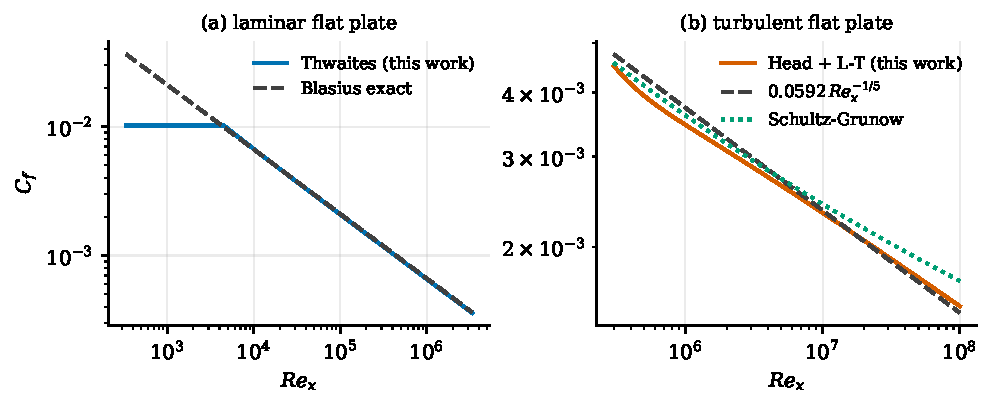
\includegraphics[width=0.98\linewidth]{fig2_verification.pdf}
  \caption{IBL verification. (a) laminar flat plate vs.\ Blasius;
  (b) turbulent flat plate vs.\ the $1/7$-power law and Schultz--Grunow.}
  \label{fig:verification}
\end{figure}

\subsection{Smith analytic limit}

With an ideal fan, no distortion, low Mach and full ingestion at the
self-propelled condition, the comparator must collapse onto the closed-form
ledger of Section~\ref{sec:unification}. It does: across power-law
exponents $n\in\{5,7,9\}$ the maximum deviation is \numSmithErr\ (target
$\le2\,\%$) --- the comparator and the closed form are the same algebra
evaluated through different code paths, so the agreement verifies the
implementation rather than the physics.

\subsection{D8 wind-tunnel benefit}

The D8 measurement \citep{uranga2017} is reproduced as a D8-like equivalent
body of revolution at 1:11 tunnel scale ($Re_L=7.2\times10^6$, tripped),
ingesting $f_\Phi=0.40$ of the fuselage boundary-layer dissipation
\citep{hall2017}, at the self-propelled condition with the FPR solved
(\numDEightFPR) so the propulsors tow the rest of the airframe.
Figure~\ref{fig:d8} compares the resulting decomposition with the
measurement. The model gives $\mathrm{PSC}=\numDEightPSC$ against
$8.2\pm0.8$\,\%, i.e.\ $+0.7$ points above the experimental band, with a
clean mechanistic diagnosis. The low-order fan re-energizes the captured
profile to a uniform jet total pressure --- a structural
$\eta_{\mathrm{fill}}=1$ idealization --- so the jet term (\numDEightJet)
overpredicts the measured 5.2\,\%; the model resolves no fan--airframe
pressure coupling, so the measured 2.4\,\% \emph{surface} contribution is
identically absent; the two errors partially cancel. We consider a
low-order model that lands within 1.6 points of a wind-tunnel measurement
\emph{with an explanation of the sign and mechanism of its error} more
useful to a designer than a tuned match.

\begin{figure}[t]
  \centering
  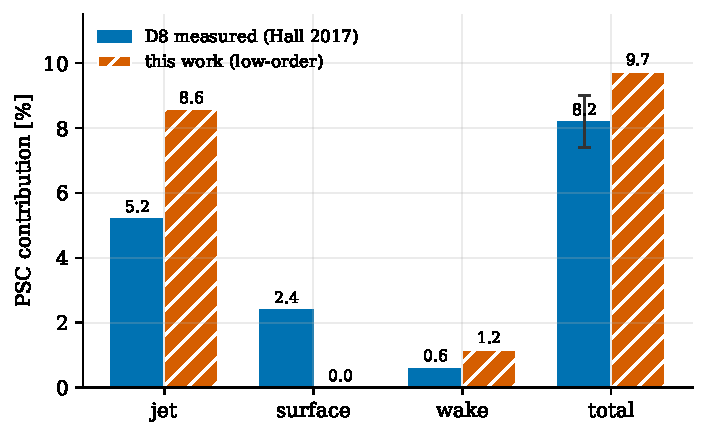
\includegraphics[width=0.62\linewidth]{fig3_d8_decomposition.pdf}
  \caption{D8 dissipation decomposition: this work vs.\ the measurement of
  \citet{uranga2017} as decomposed by \citet{hall2017}.}
  \label{fig:d8}
\end{figure}

\subsection{STARC-ABL bracket}

At the SPEC baseline with the aft fan carrying one third of cruise thrust
($D_{\mathrm{total}}=\numStarcDtot$\,kN, fuselage \numStarcDfus\,kN), the
force-driven comparator captures $f_\Phi=\numStarcFphi$ and returns a
subsystem $\mathrm{PSC}$ of \numStarcPSC\ ($P_K$ basis; \numStarcPSCshaft\
on shaft power) --- of the same order as, though 2--3 points above, the
11--12\,\% aerodynamic estimates of
the original concept study \citep{welstead2016}. Converted to aircraft
level by Eq.~\eqref{eq:netpsc}: with a mechanical drive the net power
saving is \numStarcNetMech\ (cf.\ 2.1--2.3\,\% from coupled RANS
optimization \citep{yildirim2022}, which resolves installation and coupling
losses our model idealizes away); with the turboelectric chain it is
\numStarcNetElec, and the 3500-nmi block-fuel delta is \numStarcFuel\
(snowball 1.35; \numStarcFuelNoSnow\ without). The published record spans
Giannakakis' $+1.7\pm1.0$\,\% \emph{penalty} \citep{giannakakis2020} to
NASA's $-3.4$\,\% benefit \citep{felder2022} (which credits airframe
resizing beyond the propulsive saving); our estimate falls between them,
and the obsolete 12\,\% of \citet{welstead2016} is excluded by the entire
posterior distribution of Section~\ref{sec:uq}.

% -------------------------------------------------------------------------
\section{Parametric benefit atlas}\label{sec:atlas}

\begin{figure}[t]
  \centering
  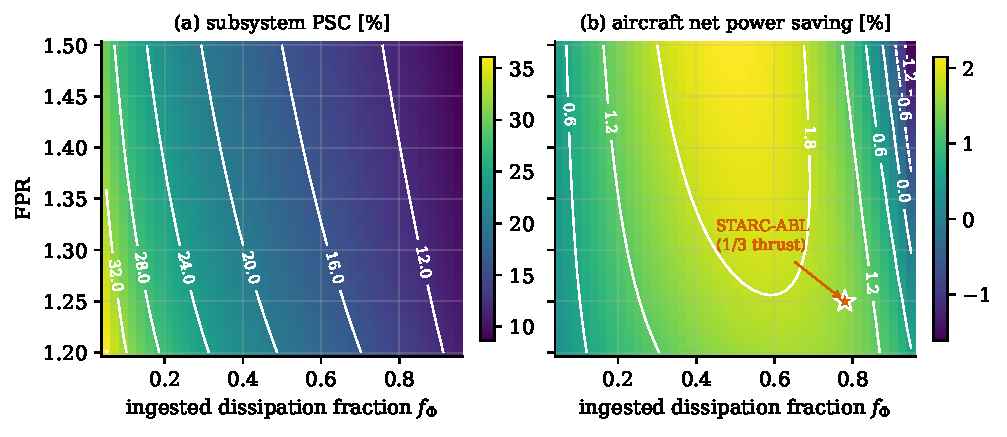
\includegraphics[width=0.98\linewidth]{fig4_heatmap.pdf}
  \caption{Benefit atlas at the cruise baseline. (a) subsystem PSC and
  (b) aircraft-level net power saving (turboelectric,
  $\eta_{\mathrm{elec}}=0.92$) over ingestion fraction and FPR; the star
  marks the STARC-ABL one-third-thrust operating point.}
  \label{fig:heatmap}
\end{figure}

Figure~\ref{fig:heatmap} maps the two headline metrics over
$(f_\Phi, \mathrm{FPR})$; all $41\times41$ cells carry validity flags from
the boundary-layer solver (none are violated at the cruise baseline; the
flags matter for off-design fineness/Mach corners of the extended maps in
the repository). Two structural features deserve emphasis because they
reconcile apparently conflicting intuitions in the literature.

\paragraph{The dilution effect.} The \emph{subsystem} PSC ---
saving per unit of that propulsor's podded-twin power --- \emph{decreases}
monotonically with $f_\Phi$ at fixed FPR. The reason is bookkeeping, not
physics: each marginal slice of captured boundary layer is faster and less
degraded than the last (Eq.~\eqref{eq:fphi} weights the deep, slow fluid
most), while the podded twin grows in proportion to the captured force
share, so the \emph{ratio} dilutes even as the \emph{absolute} saving
grows. Comparisons of PSC values across studies that sized their propulsors
differently are therefore not comparisons of the same quantity --- a
concrete instance of the reviews' reconciliation warning
\citep{moirou2023, ma2025}.

\paragraph{Diminishing returns and the interior optimum.} The
aircraft-level \emph{absolute} saving (Fig.~\ref{fig:saturation}a) grows
sublinearly but only mildly so (the $f_\Phi$ 0.2$\to$0.4 increment exceeds
the 0.6$\to$0.8 increment by $\sim$12\,\% at FPR 1.30): on the raw energy
ledger, deeper ingestion keeps paying. The \emph{net} metric does not.
Charged with the distortion penalty and the dilution of marginal capture
quality, the net power saving exhibits a sharp interior optimum
(Fig.~\ref{fig:heatmap}b): at FPR 1.30 it peaks at 1.9\,\% near
$f_\Phi=0.57$ and collapses to \emph{zero} at $f_\Phi=0.95$; at FPR 1.45
full ingestion is a net penalty of $-1.2$\,\%. The design folklore that a
BLI installation should swallow ``most'' of the layer is therefore only
half right: it should swallow \emph{about half to two thirds}, and chasing
the last quartile actively destroys benefit at realistic distortion
sensitivities. The force-driven design curves (Fig.~\ref{fig:saturation}b)
show the same physics from the designer's side: at fixed thrust share,
lowering FPR grows the capture and the subsystem PSC together, tracing the
practical design trade.

\begin{figure}[t]
  \centering
  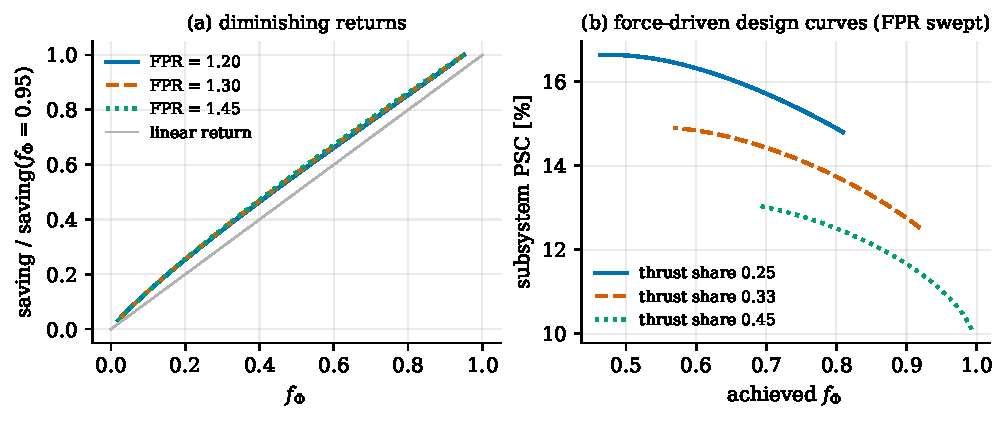
\includegraphics[width=0.98\linewidth]{fig5_saturation.pdf}
  \caption{(a) Diminishing returns of ingestion: aircraft-level saving
  normalized by its $f_\Phi=0.95$ value. (b) Force-driven design curves at
  fixed thrust share, FPR swept.}
  \label{fig:saturation}
\end{figure}

Secondary sweeps (archived with the atlas data) show mild trends with Mach
(PSC rises $\sim$1 point from $M0.72$ to $M0.82$, tracking the growth of
the recoverable fuselage dissipation with cruise speed; the compressibility
penalty on inlet recovery is second-order over this range), altitude
(weak), and fuselage fineness (slender bodies give thinner layers relative
to the hub and lower absolute savings).

% -------------------------------------------------------------------------
\section{Global sensitivity and uncertainty}\label{sec:uq}

\subsection{Input space and machinery}

Seven inputs span the design and uncertainty space (Table~\ref{tab:inputs});
design variables carry uniform distributions over their ranges, uncertain
technology/physics parameters truncated normals per the NASA reference
values and the distortion literature. Saltelli-sampled Sobol' indices
\citep{sobol2001, saltelli2010, herman2017} are computed at base sample
$N=2^{14}$ ($147\,456$ evaluations under the first/total-order Saltelli
scheme; an $N=1024$ pilot reproduces every
ranking within its confidence intervals), cross-checked against an order-3
polynomial-chaos surrogate \citep{feinberg2015} fitted on a Sobol-sequence
design and evaluated by $10^4$-sample Monte Carlo for the percentile
bands. The two independent estimates of the total-order
rankings agree on the dominant parameters for all three outputs.

\begin{table}[t]
\centering\small
\caption{UQ input space (SPEC.md \S4).}
\label{tab:inputs}
\begin{tabular}{llll}
\toprule
input & role & distribution & range/params \\
\midrule
$f_\Phi$ & design & uniform & [0.10, 0.90] \\
FPR & design & uniform & [1.20, 1.50] \\
$x_{tr}/L$ & uncertainty & uniform & [0.01, 0.10] \\
$n$ (profile) & uncertainty & trunc.\ normal & $\mathcal N(7,1)$, [4, 11] \\
$\eta_{\mathrm{pol}}$ & technology & trunc.\ normal & $\mathcal N(0.92, 0.02)$ \\
$k_{\mathrm{dist}}$ & technology & uniform & [0.00, 0.05] \\
$\eta_{\mathrm{elec}}$ & technology & trunc.\ normal & $\mathcal N(0.92, 0.02)$ \\
\bottomrule
\end{tabular}
\end{table}

\subsection{What controls the benefit}

Figure~\ref{fig:sobol} ranks the total-order indices. For the
\emph{aerodynamic} subsystem PSC, the design variable dominates as expected
($f_\Phi$: $S_T=\numSobolAeroTopVal$), with the fan-face profile exponent
$n$ --- a pure uncertainty about what shape of layer actually arrives at
the fan --- a strong second (\numSobolAeroSecondVal). But for the outputs a
program manager actually buys --- net power saving and block fuel --- the
picture changes qualitatively: the electrical-chain efficiency
$\eta_{\mathrm{elec}}$ --- a pure technology uncertainty --- rises to a
statistical tie with the ingestion design lever itself as the largest
contributor ($S_T=\numSobolNetTopVal$ each at production sampling,
$N=2^{14}$), with profile shape ($n$: 0.20) and the distortion slope
($k_{\mathrm{dist}}$: 0.12) each outranking the FPR design choice (0.07).

The claim sharpens under conditioning. Restricting the design space to
installations that already capture at least half the available dissipation
($f_\Phi\in[0.5, 0.9]$; a separate Saltelli pass on the restricted space),
the ingestion fraction's total-order index for net benefit collapses to
\numSobolCondFphi\ --- comparable to the profile-shape uncertainty
(\numSobolCondN) and barely a third of the electrical chain's
\numSobolCondElec. Once the installation swallows roughly half the layer,
\emph{the variance of the delivered benefit is governed by the electrical
chain and by profile/distortion uncertainty, not by how much more boundary
layer the designer manages to ingest}. This is the paper's central
quantitative finding, and it reframes priorities: a point of
electrical-chain efficiency is worth more to the net benefit's confidence
interval than a decile of additional ingestion.

\begin{figure}[t]
  \centering
  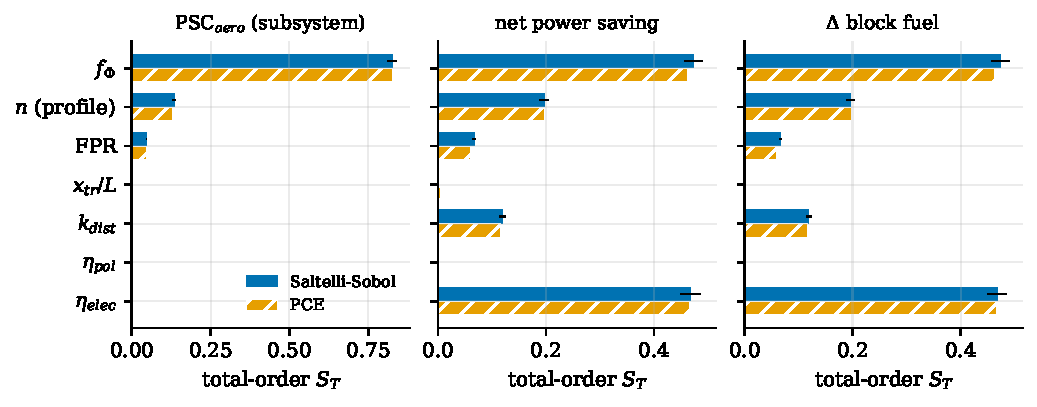
\includegraphics[width=0.98\linewidth]{fig6_sobol.pdf}
  \caption{Total-order Sobol' indices per output, Saltelli/SALib vs.\ the
  PCE cross-check.}
  \label{fig:sobol}
\end{figure}

\subsection{Distribution of the benefit}

Figure~\ref{fig:uqhist} shows the output distributions over the full input
space. The subsystem aerodynamic PSC has median \numUQPscPmed\ with a
5--95\,\% band of [\numUQPscPlo, \numUQPscPhi]. The overlaid D8
measurement (8.2\,\%) lies \emph{below} this band --- deliberately so: it
was measured under a different rule (self-propelled whole-model power) on
a different configuration, and its position outside a distribution
computed under the subsystem convention at cruise is itself a
quantitative illustration of how far bookkeeping conventions alone move
the ``BLI benefit'' (Section~\ref{sec:atlas}). Net block fuel at
3000\,nmi has
median \numUQFuelPmed\ with band [\numUQFuelPlo, \numUQFuelPhi]: the
distribution overlaps NASA's $-3.4$\,\% only in its favorable tail,
comfortably contains typical 1--3\,\% estimates, and --- notably ---
approaches zero benefit at the unfavorable end, quantifying exactly the
warning of \citet{giannakakis2020} without requiring their mass bookkeeping
to reach it. The obsolete 12\,\% early estimate lies far outside the
support everywhere.

\begin{figure}[t]
  \centering
  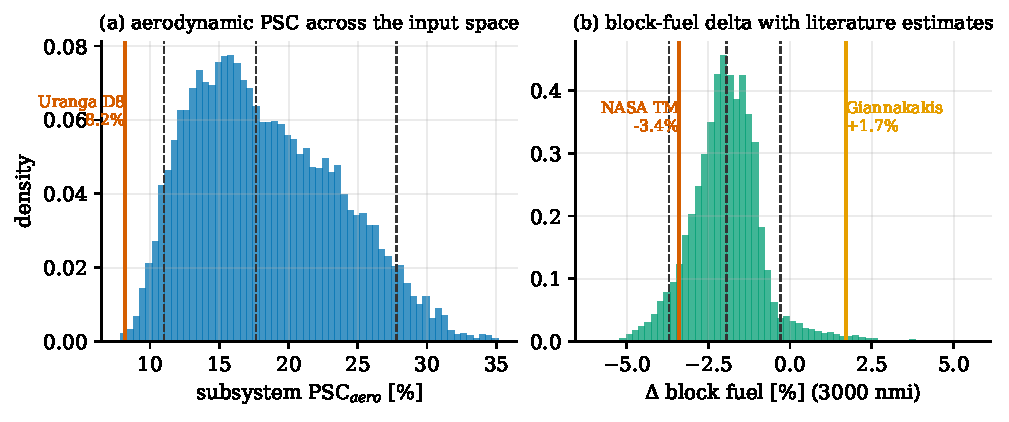
\includegraphics[width=0.98\linewidth]{fig7_uq_histograms.pdf}
  \caption{Monte-Carlo output distributions (PCE surrogate, $10^4$ LHS)
  with 5/50/95 percentiles and published point estimates overlaid.}
  \label{fig:uqhist}
\end{figure}

\begin{figure}[t]
  \centering
  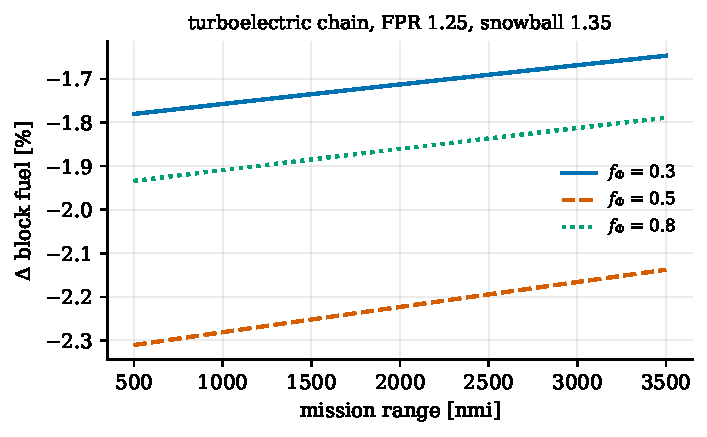
\includegraphics[width=0.62\linewidth]{fig8_fuel_vs_range.pdf}
  \caption{Block-fuel delta vs.\ mission range at three ingestion
  fractions (turboelectric chain, FPR 1.25).}
  \label{fig:fuelrange}
\end{figure}

Figure~\ref{fig:fuelrange} completes the mission view: the relative
block-fuel saving is nearly range-flat (Breguet's exponent is small over
single-aisle ranges), so the benefit case for BLI on this class rests on
the power ledger, not on mission-length leverage.

% -------------------------------------------------------------------------
\section{Discussion and limitations}\label{sec:discussion}

\paragraph{Relation to high-fidelity results.} The model's STARC-ABL
mechanical-drive net saving (\numStarcNetMech) exceeds the 2.1--2.3\,\% of
coupled RANS/cycle optimization \citep{yildirim2022} in the direction and
rough magnitude expected from its idealizations: no nacelle/installation
drag, no aft-body recontouring loss, perfect annular capture, and the
$\eta_{\mathrm{fill}}=1$ fan. The D8 comparison bounds the same
idealizations at tunnel scale ($+1.5$ points). We therefore read the
low-order model as a fast, transparent \emph{upper-envelope generator with
quantified spread}, complementary to CFD point studies: it cannot replace
a coupled solution for a specific design, but it maps where in the design
space the coupled solutions are worth buying, and how much of any promised
benefit is exposed to which uncertainty.

\paragraph{Limitations.} (i) The fan-suction \emph{surface} dissipation
term --- 2.4 points of the D8's 8.2 --- requires coupled aero-propulsive
analysis and is structurally absent; our benefit decomposition is
correspondingly conservative on that mechanism while optimistic on jet
refill. (ii) The boundary layer is axisymmetric with a power-law fan-face
surrogate; real installations ingest three-dimensional, distorted layers
(the $n$ and $k_{\mathrm{dist}}$ inputs are the low-order proxies, and the
Sobol' analysis shows they matter --- which is itself an argument for
better characterization, not merely a caveat). (iii) Ludwieg--Tillmann
underpredicts absolute skin friction at cruise $Re_\theta$ by up to
$\sim$10\,\% (bounded in CI); the PSC ratio is insensitive but absolute
dissipation figures inherit the bias. (iv) No installed-mass, trim, or
noise accounting: the mission deltas isolate the propulsive mechanism under
a fixed snowball factor. (v) Transition location is treated as an input
uncertainty rather than predicted. Each limitation is visible in the code
as an explicit assumption with a test or a UQ variable attached, which is
the posture we believe low-order aircraft analysis should adopt generally.

\paragraph{When the low-order tool suffices.} For concept screening,
technology-sensitivity ranking, and uncertainty budgeting, the model's
$\sim$3\,ms evaluations and exact bookkeeping make it strictly more
informative than point estimates quoted without uncertainty. For absolute
performance guarantees on a specific outer mold line, it does not replace
coupled CFD --- and the validation section quantifies by how much.

% -------------------------------------------------------------------------
\section{Conclusions}\label{sec:conclusions}

An open-source, tested implementation of the Drela power-balance BLI
benefit model --- unifying Smith's closed forms and Hall's decomposition,
with an exact bookkeeping identity enforced in CI --- has been used to
produce, to our knowledge, the first formal global sensitivity and
uncertainty quantification
of the BLI benefit. Three results carry practical weight. First, the
validation posture works: the model reproduces the Smith limit exactly,
lands within 1.6 points of the D8 measurement with a mechanistic account of
the difference, and brackets the modern STARC-ABL assessments while
excluding the obsolete early estimate. Second, the benefit's bookkeeping
conventions are not interchangeable: the per-propulsor PSC \emph{falls}
with ingestion fraction by dilution, the raw aircraft-level saving grows
sublinearly, and the net saving peaks near $f_\Phi\approx0.55$ before
collapsing --- full ingestion is a net penalty at realistic distortion
sensitivities --- so cross-study comparisons must state their rule, and
our atlas provides all three views. Third, and centrally: across the
credible input space the 5--95\,\% band of net block fuel is
[\numUQFuelPlo, \numUQFuelPhi], and once $f_\Phi\gtrsim0.5$ its variance
is dominated by electrical-chain efficiency ($S_T=\numSobolCondElec$) and
fan-face profile/distortion uncertainty (\numSobolCondN,
\numSobolCondKdist) rather than by ingestion fraction
(\numSobolCondFphi). The next percentage point of
confident BLI benefit is more likely to come from transmission efficiency
and inlet-distortion characterization than from more aggressive ingestion
--- a conclusion only a systematic parametric-plus-UQ study could
establish, and one now reproducible by anyone from the archived pipeline.

% -------------------------------------------------------------------------
\section*{Acknowledgments}
Portions of the implementation and manuscript were drafted with an AI
assistant (Claude, Anthropic) under human direction; the authors reviewed
and are responsible for all content. The complete build-session transcript
is archived with the repository for provenance.

\section*{Data availability}
All code, cached study data, and figure-generation scripts are available
at \url{https://github.com/abc000cool/bli-power-balance} (BSD-3-Clause),
archived at \href{https://doi.org/10.5281/zenodo.21434699}{doi:10.5281/zenodo.21434699}
(v0.1.0).
Every figure and quantitative claim regenerates via
\texttt{uv sync \&\& pytest} followed by the scripts in
\texttt{studies/} and \texttt{validation/}.

% -------------------------------------------------------------------------
\appendix

\section{Exact bookkeeping identity}\label{app:identity}

For any capture with mass flow $\dot m$, velocity profile $u(A)$ over the
capture area, and uniform fully-expanded jet $V_j'$, define the defect
integrals
$\dot D_{\mathrm{ing}}=\rho\!\int u(V_\infty-u)\,dA$,
$\dot E_{a}=\tfrac{\rho}{2}\!\int u(V_\infty-u)^2 dA$, and
$\dot E_{\mathrm{exc}}=\tfrac{\rho}{2}\!\int u(u^2-V_\infty^2)\,dA$.
The pointwise algebraic identity
$u(u^2-V_\infty^2) = -2V_\infty u(V_\infty-u) + u(V_\infty-u)^2$
integrates to
\begin{equation}
  -\dot E_{\mathrm{exc}} = V_\infty \dot D_{\mathrm{ing}} - \dot E_{a}.
  \label{eq:defectidentity}
\end{equation}
With $P_{K,\mathrm{BLI}} = \tfrac12\dot m(V_j'^2-V_\infty^2) -
\dot E_{\mathrm{exc}}$ and the expansion $\tfrac12\dot m(V_j'^2-V_\infty^2)
= \dot m(V_j'-V_\infty)V_\infty + \tfrac12\dot m(V_j'-V_\infty)^2$,
\begin{equation}
  P_{K,\mathrm{BLI}} = \left[S + \dot D_{\mathrm{res}}\right]V_\infty
  + \Phi_{\mathrm{jet}}^{\mathrm{BLI}}
  + V_\infty \dot D_{\mathrm{ing}} - \dot E_{a,\mathrm{ing}}
  = S V_\infty + \dot D_{\mathrm{full}} V_\infty
  + \Phi_{\mathrm{jet}}^{\mathrm{BLI}} - \dot E_{a,\mathrm{ing}},
\end{equation}
using the far-field force $S = \dot m(V_j'-V_\infty) - \dot
D_{\mathrm{res}}$ and $\dot D_{\mathrm{res}}+\dot D_{\mathrm{ing}}=\dot
D_{\mathrm{full}}$. The podded case at equal force, with clean inflow
($\dot E_{\mathrm{exc}}=0$) and $\dot m_{\mathrm{pod}}(V_j-V_\infty) = S +
\dot D_{\mathrm{full}}$, gives identically
$P_{K,\mathrm{pod}} = S V_\infty + \dot D_{\mathrm{full}} V_\infty +
\Phi_{\mathrm{jet}}^{\mathrm{pod}}$. Subtracting yields
Eq.~\eqref{eq:ledger}. No property of the fan model is used beyond the
existence of the jet velocities, so the identity holds exactly for the
compressible fan with losses and distortion penalties, and is asserted at
every evaluation.

\section{Nomenclature and ingestion-fraction conventions}\label{app:conventions}

Four ingestion-fraction conventions circulate; for the baseline
$n=7$ profile on the SPEC annulus, capture heights giving
$f_\Phi\in\{0.25, 0.50, 0.75\}$ correspond to mass fractions
$\{0.08, 0.21, 0.40\}$, momentum-defect fractions $\{0.27, 0.53, 0.77\}$
and annulus-area fractions $\{0.11, 0.25, 0.44\}$ of the layer --- the
spread across conventions exceeds a factor of three at low capture, which
alone explains much of the apparent disagreement between studies that
quote ``ingestion fraction'' without a definition. Cross-conversion
tables for other exponents regenerate with
\texttt{studies/conventions\_table.py}. All results in this paper use
$f_\Phi$ (Eq.~\eqref{eq:fphi}), the dissipation/KE-defect fraction aligned
with \citet{hall2017}.

\bibliographystyle{plainnat}
\bibliography{references}

\end{document}
